\documentclass[t, compress]{beamer}
% Defines
\def\CC{{\mathcal{C}}}
% Packages (Standard)
\usepackage[ngerman]{babel}
\usepackage[utf8]{inputenc}
\usepackage[T1]{fontenc}
\usepackage{graphicx}
\usepackage{amsmath}
\usepackage{amsfonts}
\usepackage{amssymb}
\usepackage{hyperref}
\usepackage{xcolor}
\usepackage{caption}
%\usepackage{natbib}
\usepackage{verbatim}
\usepackage{listings}
\usepackage{subfig}

%%%%%%%%%%%%%%%%%%%%%%%%%%%%%%%%%%%%%
%EIGENE INCLUDES FUER DEN 3. VORTRAG:
%%%%%%%%%%%%%%%%%%%%%%%%%%%%%%%%%%%%%
%Marc
\usepackage{mathtools}
\usepackage{dsfont}



%Eigene Befehle:
\newcommand{\rn}{\mathbb{R}}
\renewcommand{\hat}[1]{\tilde{#1}}

%EIGENE BEFEHLE FUER DEN 3. VORTRAG:
\newcommand{\bx}{\boldsymbol{x}}
\newcommand{\bv}{\boldsymbol{v}}

% Die Beamervorlage einbinden
% Farben fuer die Uni Koeln
\definecolor{unikoelndarkblue}{rgb}{0.25, 0.47, 0.61}
\definecolor{unikoelngray}{rgb}{0.89, 0.89, 0.89}
\definecolor{unikoelnlightblue}{rgb}{0.91, 0.93, 0.95}
\definecolor{unikoelndarkgray}{rgb}{0.41, 0.33, 0.33}
\definecolor{unikoelnred}{rgb}{0.85, 0.16, 0.11}
\definecolor{unikoelngreen}{rgb}{0.16, 0.85, 0.11}

% Aussehen der Folien
\mode<presentation>
{
  \defbeamertemplate*{footline}{authordateframes}
  {
   \leavevmode%
   \hbox{%
   \begin{beamercolorbox}[wd=.5\paperwidth,ht=2.25ex,dp=1ex,left]{author in head/foot}%
   \hspace*{1em}\usebeamerfont{author in head/foot}%\insertshortauthor~
   \end{beamercolorbox}%
   \begin{beamercolorbox}[wd=.5\paperwidth,ht=2.25ex,dp=1ex,right]{date in head/foot}%
     \usebeamerfont{date in head/foot}\insertshortdate{}\hspace*{2em}
     \insertframenumber{}\hspace*{2ex} 
    \end{beamercolorbox}}%
   \vskip0pt%
  }
								
  \defbeamertemplate*{headline}{miniframeslogo}
  {%
    \begin{beamercolorbox}[colsep=1.5pt]{upper separation line head}%
    \end{beamercolorbox}
    \begin{beamercolorbox}{section in head/foot}
    \vskip2pt\insertsectionnavigationhorizontal{\paperwidth}{}{\hskip0pt plus1filll}\vskip2pt
    \end{beamercolorbox}%
    \begin{beamercolorbox}[colsep=1.5pt]{lower separation line head}
    \end{beamercolorbox}
  }
			
  \useoutertheme[footline=authorinstitute]{miniframes}
  \setbeamertemplate{mini frames}[box]

  \useinnertheme{rectangles}

  \setbeamertemplate{footline}[authordateframes]
  \setbeamertemplate{headline}[miniframeslogo]
}
			
% Etwas mehr Platz schaffen			
\addtobeamertemplate{frametitle}{}{\vspace*{-0.5\baselineskip}}

% Farbschema anpassen
\setbeamertemplate{section in head/foot shaded}[default][40]
\setbeamercolor*{section in head/foot}{fg=unikoelndarkgray, bg=unikoelngray}
\setbeamercolor*{subsection in head/foot}{fg=unikoelndarkgray, bg=unikoelngray}
\setbeamercolor*{upper separation line head}{fg=white, bg=unikoelndarkblue}
\setbeamercolor*{lower separation line title}{fg=white, bg=unikoelndarkblue}
\setbeamercolor*{author in head/foot}{fg=unikoelndarkgray, bg=unikoelngray}
\setbeamercolor*{date in head/foot}{fg=unikoelndarkgray, bg=unikoelngray}
\setbeamercolor*{palette primary}{fg=unikoelndarkblue,bg=white}
\setbeamercolor*{palette secondary}{fg=white, bg=unikoelnlightblue}
\setbeamercolor*{palette tertiary}{bg=unikoelndarkblue, fg=unikoelnlightblue}
\setbeamercolor*{structure}{fg=unikoelndarkblue}
\setbeamercolor{titlelike}{parent=pallette primary, fg=unikoelndarkblue, bg=white}
\setbeamercolor{frametitle}{fg=unikoelndarkblue, bg=white}
\setbeamercolor{block title}{fg=unikoelndarkblue, bg=white}
\setbeamercolor{block body}{fg=unikoelndarkgray, bg=white}
\setbeamercolor{block body}{fg=unikoelndarkgray, bg=white}
\setbeamercolor{block title example}{fg=white, bg=unikoelndarkblue}
\setbeamercolor{block body example}{bg=unikoelngray}						
\setbeamercolor{block title alerted}{fg=white, bg=unikoelnred}
\setbeamercolor{block body alerted}{bg=unikoelngray}
\setbeamercolor{alerted text}{fg=unikoelnred}
\setbeamercolor{example text}{fg=unikoelndarkblue}
                
% Fix fuer komisch ausgerichtete Spalten in Frames mit top-align
\makeatletter      
 \define@key{beamerframe}{t}[true]{% top
   \beamer@frametopskip=.2cm plus .5\paperheight\relax%
   \beamer@framebottomskip=0pt plus 1fill\relax%
   \beamer@frametopskipautobreak=\beamer@frametopskip\relax%
   \beamer@framebottomskipautobreak=\beamer@framebottomskip\relax%
   \def\beamer@initfirstlineunskip{}%
 }
\makeatother  

% Ein paar nuetzliche Beamermakros

\newenvironment{itemblock}[1]{%
	\begin{block}{#1}
		\begin{itemize}
}{%
		\end{itemize}
	\end{block}
}

\newenvironment{alitemblock}[1]{%
	\begin{alertblock}{#1}
		\begin{itemize}
}{%
		\end{itemize}
	\end{alertblock}
}

\newenvironment{exitemblock}[1]{%
	\begin{exampleblock}{#1}
		\begin{itemize}
}{%
		\end{itemize}
	\end{exampleblock}
}

		\newenvironment{enumblock}[1]{%
	\begin{block}{#1}
		\begin{enumerate}
}{%
		\end{enumerate}
	\end{block}
}

\newenvironment{alenumblock}[1]{%
	\begin{alertblock}{#1}
		\begin{enumerate}
}{%
		\end{enumerate}
	\end{alertblock}
}

\newenvironment{exenumblock}[1]{%
	\begin{exampleblock}{#1}
		\begin{enumerate}
}{%
		\end{enumerate}
	\end{exampleblock}
}

\newenvironment{mycolumns}{%
	\vspace*{-0.5\baselineskip}
	\begin{columns}[T, onlytextwidth]
}{%
	\end{columns}
}

\newcommand{\str}{\structure}


% Zum debuggen nuetzlich: Erzeugt ein Gitter im Hintergrund
%\setbeamertemplate{background}[grid][step=0.5cm]

% Navigationssymbole ausblenden
\setbeamertemplate{navigation symbols}{}

% Metadaten
\title{Relevance Propagation for Deep Neural Networks}
\subtitle{Zwischenvortrag 3}
\author{Theo Conrads, Robin K\"uhling, Marc Bremser}
\date{\today} 
\titlegraphic{\includegraphics[width=5cm]{grafiken_marc/titlegraphic.png}}

% Der eigentliche Vortrag  
\begin{document}


\begin{frame}
	\titlepage
\end{frame}

\begin{frame}{Überblick}
  \tableofcontents[hideallsubsections]
\end{frame}

\section{Einleitung}
\begin{frame}{Aufgaben}
\begin{large}
\begin{center}
\vspace*{1cm}
\begin{minipage}{0.9\textwidth}
\begin{enumerate}
\item \textbf{Arbeit an einem CNN für den Pascal VOC 2012 Datensatz fortsetzen}
\vspace*{10pt}
\item \textbf{Implementierung des Ansatz der Deep Taylor Decomposition für DNN (insbesondere CNN)}
\vspace*{0pt}
\item \textbf{Vergleich LRP $\leftrightarrow$ Deep Taylor Decomposition}
\end{enumerate}
\end{minipage}
\end{center}
\end{large}
\end{frame}

\section{Implementierung eines CNN für den Pascal VOC}
\begin{frame}{Implementierung eines CNN für den Pascal VOC}
\begin{enumerate}
\item Das VGG-Modell
\item Finetuning
\item Regularisierung
\item Ein eigener Model Checkpoint
\item Vergleich von Ergebnissen
\end{enumerate}
\end{frame}

\begin{frame}{Das VGG-Modell}
\includegraphics[scale=0.3]{./grafiken_robin/vgg16.png}
\end{frame}

\begin{frame}{Finetuning}
Wir entfernen die Dense Layer aus dem bereits trainierten VGG16 und trainieren diese neu\\
\vspace*{0.5cm}
\includegraphics[scale=0.4]{./grafiken_robin/finetuning.png}
\end{frame}

\begin{frame}{Regularisierung}
\begin{itemize}
\item Hier besoners wichtig weil: 
\begin{enumerate}
\item der Datensatz klein ist
\item die Klassen ungleich viele Bilder enthalten
\end{enumerate}
\item Methoden:
\begin{enumerate}
\item Dropout
\item BatchNormalization
\item Data Augmentation
\item Sample anderer Klassen
\end{enumerate}
\end{itemize}
\end{frame}

\begin{frame}{Regularisierung}
\begin{itemize}
\item Data Augmentation
\begin{itemize}
\item Idee: Erweitern des Datensatzes um Generalisierungseigenschatfen und Performance des NN zu verbessern
\item Umsetzung: Zufällige Modifzierzungen der Bilder im Datenstrom zur Laufzeit
\item Implmentierung: mittels der Klasse ImageDataGenerator von Keras
\end{itemize}
\end{itemize}
\end{frame}

\begin{frame}{Regularisierung}
\begin{itemize}
\item Data Augmentation
\begin{itemize}
\item Beispiele:
\end{itemize}
\end{itemize}
\begin{figure}
\stackunder[5pt]{\includegraphics[scale=0.3]{./grafiken_robin/horizontal_flip.png}}{Horizontal Flip}%
\hspace{1cm}%
\stackunder[5pt]{\includegraphics[scale=0.3]{./grafiken_robin/brightness.png}}{Brightness Range}
\caption{}
\end{figure}
\footnote{Quelle: https://machinelearningmastery.com/how-to-configure-image-data-augmentation-when-training-deep-learning-neural-networks/}
\end{frame}

\begin{frame}{Sample anderer Klasses}
\begin{itemize}
\item Ein NN muss lerenen was zu einer Klasse gehört und was nicht
\item Problem: Falsche Entscheidungen für eine Klasse anhand von Merkmalen die Häufig mit dieser Klasse auftreten
\item Idee: Hinzufügen von Bildern die keine der zu trainierenden Klassen enhalten
\end{itemize}
\end{frame}

\begin{frame}{Ein eigener Model Checkpoint}
\begin{itemize}
\item Idee: Speichere das Model nicht zum Zeitpunkt minimalen Fehlers sondern anhand spezieller Metriken
\begin{enumerate}
\item Precision: 
\begin{align*}
&\frac{true\_positives}{true\_positives + false\_positives}\\
&\text{Welcher Anteil positiv vorhergesagter Label war korrekt?}
\end{align*}
\item Recall:
\begin{align*}
&\frac{true\_positives}{true\_positives + false\_negatives}\\
&\text{Welcher Anteil positiver Label wurde korrekt vorhergesagt?}
\end{align*}
\end{enumerate}
\end{itemize}
\end{frame}

\begin{frame}{Ein eigener Model Checkpoint}
\begin{itemize}
\item Ziel: beide möglichst groß mit ähnlicher Größenordnung
\item Implementierung: Speichere das Modell falls
\begin{enumerate}
\item mind. eine Metrik sich verbessert hat wärend die andere nicht schlechter geworden ist
\item die Metriken im Mittel besser geworden sind und ihr Abstand sich verringert hat
\end{enumerate}
\end{itemize}
\end{frame}

\begin{frame}{Vergleich der Ergebnisse}
\begin{itemize}
\item Das Modell für 2 Klassen
\item Klassen = Person, Pferd
\includegraphics[scale=0.06]{./grafiken_robin/person_horse_plots.png}
\end{itemize}
\end{frame}

\begin{frame}{Vergleich der Ergebnisse}
\begin{itemize}
\item Das Model für 5 Klassen
\item Klassen = Katze, Esstisch, Person, Flugzeug, Flasche
\includegraphics[scale=0.06]{./grafiken_robin/several_classes_plots.png}
\end{itemize}
\end{frame}



\section{Taylor Decomposition}
\frame{\sectionpage}
\frame{\frametitle{Taylor Decomposition - Rückblick}
\begin{itemize}
\item Einfaches Netzwerk mit einem Hidden Layer, ReLU Aktivierung und Sum-Pooling als Output.
\item Zusätzliche Voraussetzung: $b_j \leq 0$. 
\begin{figure}[H]
\includegraphics[width = 0.7 \textwidth]{grafiken_marc/simple_net.png}
\end{figure}
\item Für das Outputneuron $x_k$ gilt: $x_k = max(0,\sum_{j} x_j)$
%\item Gesucht ist eine Vorschrift, nach der die Relevanz $R_k$ auf die Neuronen der vorherigen Schicht verteilt wird.
\end{itemize}
}

\frame{\frametitle{Taylor Decomposition - Rückblick}
\begin{itemize}
\item Suche eine Nullstelle f\"ur die Taylorentwicklung von $R_k(\boldsymbol{x}) = \sum_j x_j$.

\begin{figure}
\includegraphics[width = 0.6\textwidth]{grafiken_marc/rel_prop_1.png}
\end{figure}
\pause
\item Wg. ReLU Aktivierung im vorherigen Layer und $\sum_j x_j \overset{!}{=} 0$ ist $\tilde{\boldsymbol{x}}=$\textbf{0} die einzige Nullstelle von $R_k$.
\item Wegen $R_j=\frac{\partial R_{k}}{\partial x_{j}}(x_j - \tilde{x}_j)=1 \cdot (x_j - 0)$ gilt also
\item $R_{j}=x_{j}= \max \left(0, \sum_{i} x_{i} w_{i j}+b_{j}\right)$
\end{itemize}
}

\frame{\frametitle{Taylor Decomposition - Generische Regel}
\begin{itemize}
%\item Führe nun für jede der $R_j$ Taylorentwicklung mit einem eigenen Entwicklungspunkt $\hat{x}^{(j)}$ durch.
\item Es gilt $R_j = x_j = \max \left(0, \sum_{i} x_{i} w_{i j}+b_{j}\right)$

\begin{figure}
\includegraphics[width = 0.6\textwidth]{grafiken_marc/rel_prop_2.png}
\end{figure}
%\pause
\item Unterscheide nun 2 Fälle:
\begin{enumerate}
\item $R_j=0$: Nicht aktivierte Neuronen sollen keine Relevanz zurückverteilen. Insbesondere gilt hier $\tilde{\bx}= \bx $.
\item $R_j>0$: Hierfür wird ein Richtungsvektor $\bv^{(j)}$ definiert. $\tilde{\bx}$ soll von der Form $\bx	+ t \cdot \bv^{(j)}$, mit $t \in \rn$ sein.
\end{enumerate}
\end{itemize}
}


\begin{frame}{Taylor - Entwicklungspunkt}
\begin{itemize}
\item Allgemeine Vorgehensweise: 
\item Durch Einsetzen von $\tilde{\bx}=\bx	+ t \cdot \bv^{(j)}$ in die Ebenengleichung $\sum_{i} \tilde{x}_{i} w_{i j}+b_{j} = 0$ lässt sich eine allgemeine Formel für $t$ finden.
\item Somit gilt: 
\begin{align*}
0 &= \sum_{i} \left(x_{i} + t v_i^{(j)} \right) w_{i j}+b_{j} \\
\Leftrightarrow -t& =\frac{\sum_{i} x_{i} w_{i j}+b_{j}}{\sum_{i} v_{i}^{(j)} w_{i j}}\\
\ \\
\Rightarrow x_i - \tilde{x_i} &= -t v_i^{(j)} = \frac{\sum_{i} x_{i} w_{i j}+b_{j}}{\sum_{i} v_{i}^{(j)} w_{i j}} v_i^{(j)}
\end{align*}
\end{itemize}
\end{frame}

\begin{frame}{Taylor - Entwicklungspunkt}
\begin{itemize}
\item Für die Umverteilung von der $l+1$-ten Schicht in die $l$-te Schicht gilt
\begin{align*}
R_i^l &= \sum_{j} R_{i \leftarrow j}^l =  \sum_{j} \frac{\partial R_{j}^{l+1}}{\partial x_{i}^l}
(x_i - \tilde{x_i}) \\
&= \sum_{j : R_j = 0} \frac{\partial R_{j}^{l+1}}{\partial x_{i}^l} \cdot 0 + \sum_{j: R_j>0} w_{ij} \frac{\sum_{i} x_{i} w_{i j}+b_{j}}{\sum_{i} v_{i}^{(j)} w_{i j}} v_i^{(j)} \\
&= \sum_{j} \frac{v_i^{(j)}  w_{i j}}{\sum_{i} v_{i}^{(j)} w_{i j}} R_j^{l+1}
\end{align*}
\item $\Rightarrow$ Allgemeine Formel in Abhängigkeit von $v_i^{(j)}$
\end{itemize}
\end{frame}



%\section{Part 2}
\begin{frame}{Aufgabe}
\begin{itemize}
\item Herleitung $z^B$ Regel und Implementierung der einzelnen Regeln
\item Vergleich der Ergebnisse
\end{itemize}
\end{frame}

%\section{Part 2}
\begin{frame}{Erweiterung auf tiefe Netze}
\begin{itemize}
\item Bei tiefen Netzen, insbesondere Convolutional Layern ist die Relevanzfunktion nicht unbedingt explizit angegeben.
\end{itemize}
\vspace*{20pt}
\begin{minipage}{0.42\textwidth}
\includegraphics[width=\textwidth]{grafiken_marc/simple_net.png}
\end{minipage}
\begin{minipage}{0.52\textwidth}
\includegraphics[width=\textwidth]{grafiken_marc/DNN.png}
\end{minipage}
\vspace*{10pt}
\begin{itemize}
\item Ein Feature kann vorhanden sein, aber bei der Bilderkennung keine Rolle spielen
\end{itemize}
\footnote{Grafik entnommen aus \ref{itm:Mont17}}
\end{frame}

\begin{frame}{Erweiterung auf tiefe Netze}
\begin{itemize}
\item Gesucht ist eine Approximation der Relevanz Funktion, die leicht zu analysieren ist.
\item Führe das Konzept \textbf{Relevanz-Modell} ein, um bei tieferen Netzen die Relevanzfunktion $R_j^{l+1}(\bx^{l})$ zu approximieren.
\item Nehme an, die Relevanzfunktion $R_j$ lässt sich in der Form $R_j = x_j \cdot c_j$ schreiben, wobei $c_j$ konstant ist.
\item Im Paper als "{}Training Free"{} Ansatz vorgestellt
\end{itemize}
\end{frame}

\begin{frame}{Erweiterung auf tiefe Netze}
\begin{itemize}
\item Nehme an, die Relevanzfunktion $R_j$ lässt sich in der Form $R_j = x_j \cdot c_j$ schreiben, mit $c_j$ konstant.
\item Betrachte die generische Redistributionsregel
\begin{align*}
R_i &= \sum_{j} \frac{x_{i} \cdot \rho(w_{i j})}{\sum_{i} x_{i} \cdot \rho(w_{i j})} R_{j}\\
& = x_{i} \sum_{j}  \frac{ \rho(w_{i j})}{\sum_{i} x_{i} \cdot \rho(w_{i j})} x_j \cdot c_j \\
&= x_i \sum_{j}   \rho(w_{i j}) \frac{\max \left(0, \sum_{i} x_{i} w_{i j}\right)}{\sum_{i} x_{i} \cdot \rho(w_{i j})} c_j
\end{align*}
\end{itemize}
\end{frame}

\begin{frame}{Erweiterung auf tiefe Netze}
\begin{itemize}
\item Nehme an, die Relevanzfunktion $R_j$ lässt sich in der Form $R_j = x_j \cdot c_j$ schreiben, mit $c_j$ konstant.
\item Betrachte die generische Redistributionsregel
\begin{align*}
R_i &= \sum_{j} \frac{x_{i} \cdot \rho(w_{i j})}{\sum_{i} x_{i} \cdot \rho(w_{i j})} R_{j}\\
& = x_{i} \sum_{j}  \frac{ \rho(w_{i j})}{\sum_{i} x_{i} \cdot \rho(w_{i j})} x_j \cdot c_j \\
&= x_i \underbrace{\sum_{j}   \rho(w_{i j}) \frac{\max \left(0, \sum_{i} x_{i} w_{i j}\right)}{\sum_{i} x_{i} \cdot \rho(w_{i j})} c_j}_{\colonapprox c_i}
\end{align*}
\end{itemize}
\end{frame}

\begin{frame}{Erweiterung auf tiefe Netze}
\begin{itemize}
\item Es gilt also
\begin{align*}
R_i = x_i \underbrace{\sum_{j}   \rho(w_{i j}) \frac{\max \left(0, \sum_{i} x_{i} w_{i j}\right)}{\sum_{i} x_{i} \cdot \rho(w_{i j})} c_j}_{\colonapprox c_i} = \sum_{j}    \frac{\rho(w_{i j}) \cdot x_i}{\sum_{i} x_{i} \cdot \rho(w_{i j})} R_j
\end{align*}
\item D.h. $R_i^l$ lässt sich wieder schreiben als $x_i^l \cdot c_i^l$, mit $c_i^l$ annähernd konstant.
\item Ausgehend von der letzten Schicht kann die Relevanz somit auch gemäß der hergeleiteten Regeln zurück zum Input verteilt werden.
\item Der Parameter $c_i^l$ wird dabei durch die betrachtete Regel "{}induktiv"{} gebildet.
\end{itemize}
\end{frame}


\begin{frame}{Zusammenhang mit LRP}
\begin{itemize}
\item Die klassische $LRP-0$ Formel kann als Deep Taylor Entwicklung im Nullpunkt gesehen werden
\item Betrachte O.B.d.A. ein Neuron $x_j$ mit $R_j > 0$. 
\item Die Suchrichtung $\bv$ ist hierbei der Punkt $\bx$ selbst, und somit gilt:
\pause
\begin{align*}
R_{i \leftarrow j}^l &=\frac{\partial R_{j}^{l+1}}{\partial x_{i}^l}
(x_i - \tilde{x_i})  = w_{ij} \cdot c_j \cdot (x_i - \tilde{x_i}) \\
&= w_{ij} \cdot c_j \cdot \frac{\sum_{i} x_{i} w_{i j}+b_{j}}{\sum_{i} x_{i} w_{i j}} x_i\\
&= \frac{x_i \cdot w_{ij}}{\sum_{i} x_{i} w_{i j}} x_j \cdot c_j
\end{align*}
\end{itemize}
\end{frame}


\begin{frame}{Zusammenhang mit LRP}
\begin{itemize}
\item Die klassische $LRP-0$ Formel kann als Deep Taylor Entwicklung im Nullpunkt gesehen werden
\item Betrachte O.B.d.A. ein Neuron $x_j^{l+1}$ mit $R_j > 0$. 
\item Die Suchrichtung $\bv$ ist hierbei der Punkt $\bx$ selbst, und somit gilt:
\begin{align*}
R_{i \leftarrow j}^l &=\frac{\partial R_{j}^{l+1}}{\partial x_{i}^l}
(x_i - \tilde{x_i})  = w_{ij} \cdot c_j \cdot (x_i - \tilde{x_i}) \\
&= w_{ij} \cdot c_j \cdot \frac{\sum_{i} x_{i} w_{i j}+b_{j}}{\sum_{i} x_{i} w_{i j}} x_i\\
&= \frac{x_i \cdot w_{ij}}{\sum_{i} x_{i} w_{i j}} \underbrace{ x_j \cdot c_j}_{ R_j }
\end{align*}
\end{itemize}
\end{frame}

\begin{frame}{Zusammenhang mit LRP}
\begin{itemize}
\item Für die totale Relevanz von $x_i$ gilt:

\begin{align*}
R_i^l = \sum_{j} R_{i \leftarrow j}^l &= \sum_{j} \frac{x_i \cdot w_{ij}}{\sum_{i} x_{i} w_{i j}} R_j^{l+1} = \sum_{j} \frac{z_{ij}}{\sum_{i} z_{i j}} R_j^{l+1}
\end{align*}
\item Mit der gleichen Vorgehensweise können auch die $LRP-\varepsilon$ Regel sowie $LRP-\gamma$ hergeleitet werden.
\item Deep Taylor Decomposition als Basis für \textit{LRP}
\item Wesentlicher Unterschied: Geforderte Konsistenz von Montavon et al. im Vergleich zu den \textit{LRP} Regeln
\end{itemize}
\end{frame}



\section{Nähere Analyse der Implementierungsergebnisse}
\frame{\sectionpage}
\begin{frame}{Wiederholung}
\begin{itemize}
\item \textbf{Konservierung} \\
Eine LRP-Regel ist \textbf{konservativ} genau dann, wenn für die Relevanzwerte der Inputschicht und jeden Input $x$ gilt:
\begin{equation*}
\sum_i R_i(x) = f(x)
\end{equation*}
\item \textbf{Positivität} \\
Eine LRP-Regel ist \textbf{positiv} genau dann, wenn gilt:
\begin{equation*}
\forall x, i \quad R_i \geq 0
\end{equation*}
\item \textbf{Konsistenz} \\
Eine LRP-Regel ist \textbf{konsistent} genau dann, wenn sie \textbf{konservativ} und \textbf{positiv} ist.
\end{itemize}
\end{frame}

\begin{frame}{LRP-0}
\begin{equation*}
R_{j}=\sum_{k} \frac{a_{j} w_{j k}}{\sum_{i} a_{i} w_{i k}} R_{k}
\end{equation*}
\begin{itemize}
\item \textbf{konservativ:} \checkmark\footnote{Gilt hier und im Folgenden nur unter der Vorussetzung, dass der Bias nicht hinzuaddiert wird. Alle Bilder des Kapitels wurden unter Verwendung des Bias erstellt.}
\item \textbf{positiv:} \hspace{0.71cm} \textbf{X}
\item \textbf{konsistent:} \hspace{0.1cm} \textbf{X}
\end{itemize}
\includegraphics[width=\textwidth]{grafiken_theo/LRP-0_Check.png}
\end{frame}

\begin{frame}{LRP-$\epsilon$}
\begin{equation*}
R_{j}=\sum_{k} \frac{a_{j} w_{j k}}{\epsilon + \sum_{i} a_{i} w_{i k}} R_{k}
\end{equation*}
\begin{itemize}
\item \textbf{konservativ:} \textbf{X}
\item \textbf{positiv:} \hspace{0.71cm} \textbf{X}
\item \textbf{konsistent:} \hspace{0.1cm} \textbf{X}
\end{itemize}
\includegraphics[width=\textwidth]{grafiken_theo/LRP-eps_Check.png}
\end{frame}

\begin{frame}{LRP-$\epsilon$ - Abhängigkeit von $\epsilon$}
\begin{itemize}
\item Mit wachsendem $\epsilon$ verteilt sich die zurückgegebene Relevanz auf weniger Pixel
\item Das Rauschen der Relevanz nimmt ab und Konturen werden deutlicher
\end{itemize}
\includegraphics[width=0.95\textwidth]{grafiken_theo/Epsilon_Entwicklung.png}
\end{frame}

\begin{frame}{LRP-$\gamma$}
\begin{equation*}
R_{j}=\sum_{k} \frac{a_{j} \cdot \left(w_{j k} + \gamma \cdot w_{i j}^+ \right)}{\sum_{i} a_{i} \cdot \left(w_{j k} + \gamma \cdot w_{i j}^+ \right)} R_{k}
\end{equation*}
\begin{itemize}
\item \textbf{konservativ:} \checkmark
\item \textbf{positiv:} \hspace{0.71cm} \textbf{X}
\item \textbf{konsistent:} \hspace{0.1cm} \textbf{X}
\end{itemize}
\includegraphics[width=\textwidth]{grafiken_theo/LRP-Gamma_Check.png}
\end{frame}

\begin{frame}{LRP-$\gamma$ - Abhängigkeit von $\gamma$}
\begin{itemize}
\item Mit wachsendem $\gamma$ verlieren negative Relevanzen an Wert
\item Bildbereiche, die nicht zum klassifizierten Objekt gehören, werden "relevanter" \\
\item Es gilt LRP-$\gamma \xrightarrow {\gamma \rightarrow \infty} z^+$-Regel
\end{itemize}
\includegraphics[width=0.95\textwidth]{grafiken_theo/Gamma_Entwicklung.png}
\end{frame}

\begin{frame}{LRP-Komposition}
\begin{itemize}
\item Kombinierte Anwendung der vorherigen drei Regeln
\item Aus den Eigenschaften der einzelnen Regeln folgt, dass die Komposition weder positiv, noch konservativ ist.
\item Subjektiv betrachtet liefert diese Regel die interpretierbarsten Visualisierungen.
\vspace{1cm}
\end{itemize}
\includegraphics[width=\textwidth]{grafiken_theo/LRP-Comp_Check.png}
\end{frame}

\begin{frame}{$z^+$-Regel}
\begin{equation*}
R_{j}=\sum_{k} \frac{a_{j} \cdot w_{i j}^+}{\sum_{i} a_{i} \cdot w_{i j}^+} R_{k}
\end{equation*}
\begin{itemize}
\item \textbf{konservativ:} \checkmark
\item \textbf{positiv:} \hspace{0.71cm} \checkmark
\item \textbf{konsistent:} \hspace{0.1cm} \checkmark
\end{itemize}
\includegraphics[width=0.9\textwidth]{grafiken_theo/z+_Check.png}
\end{frame}

\begin{frame}{Übersicht Konservierung}
\begin{figure}
\includegraphics[width=0.85\textwidth]{grafiken_theo/relative_R_plots_374.png}
\end{figure}
\end{frame}


\section{Nähere Analyse der $z^+$-Regel}
\frame{\sectionpage}
\begin{frame}{Beobachtung}
\begin{itemize}
\item Die visualisierten Erklärungen für zwei verschiedene Klassen auf einem Bild ähneln sich sehr stark.
\item Bereits im drittletzten Dense-Layer wurde die Relevanz für beide Klassifikationen auf die gleichen Neuronen verteilt.
\end{itemize}
\includegraphics[width=\textwidth]{grafiken_theo/z+_vergleich.png}
\end{frame}

\begin{frame}{Vermutung}
\begin{itemize}
\item Negative Gewichte tragen stark zur Klassifizierung eines Objektes bei.
\item Durch das Ignorieren der Gewichte geht Information verloren.
\item Markante Features, die nicht oder negativ zur Klassifizierung beitragen, werden in der Backpropagation nicht gehemmt.
\end{itemize}
\begin{figure}
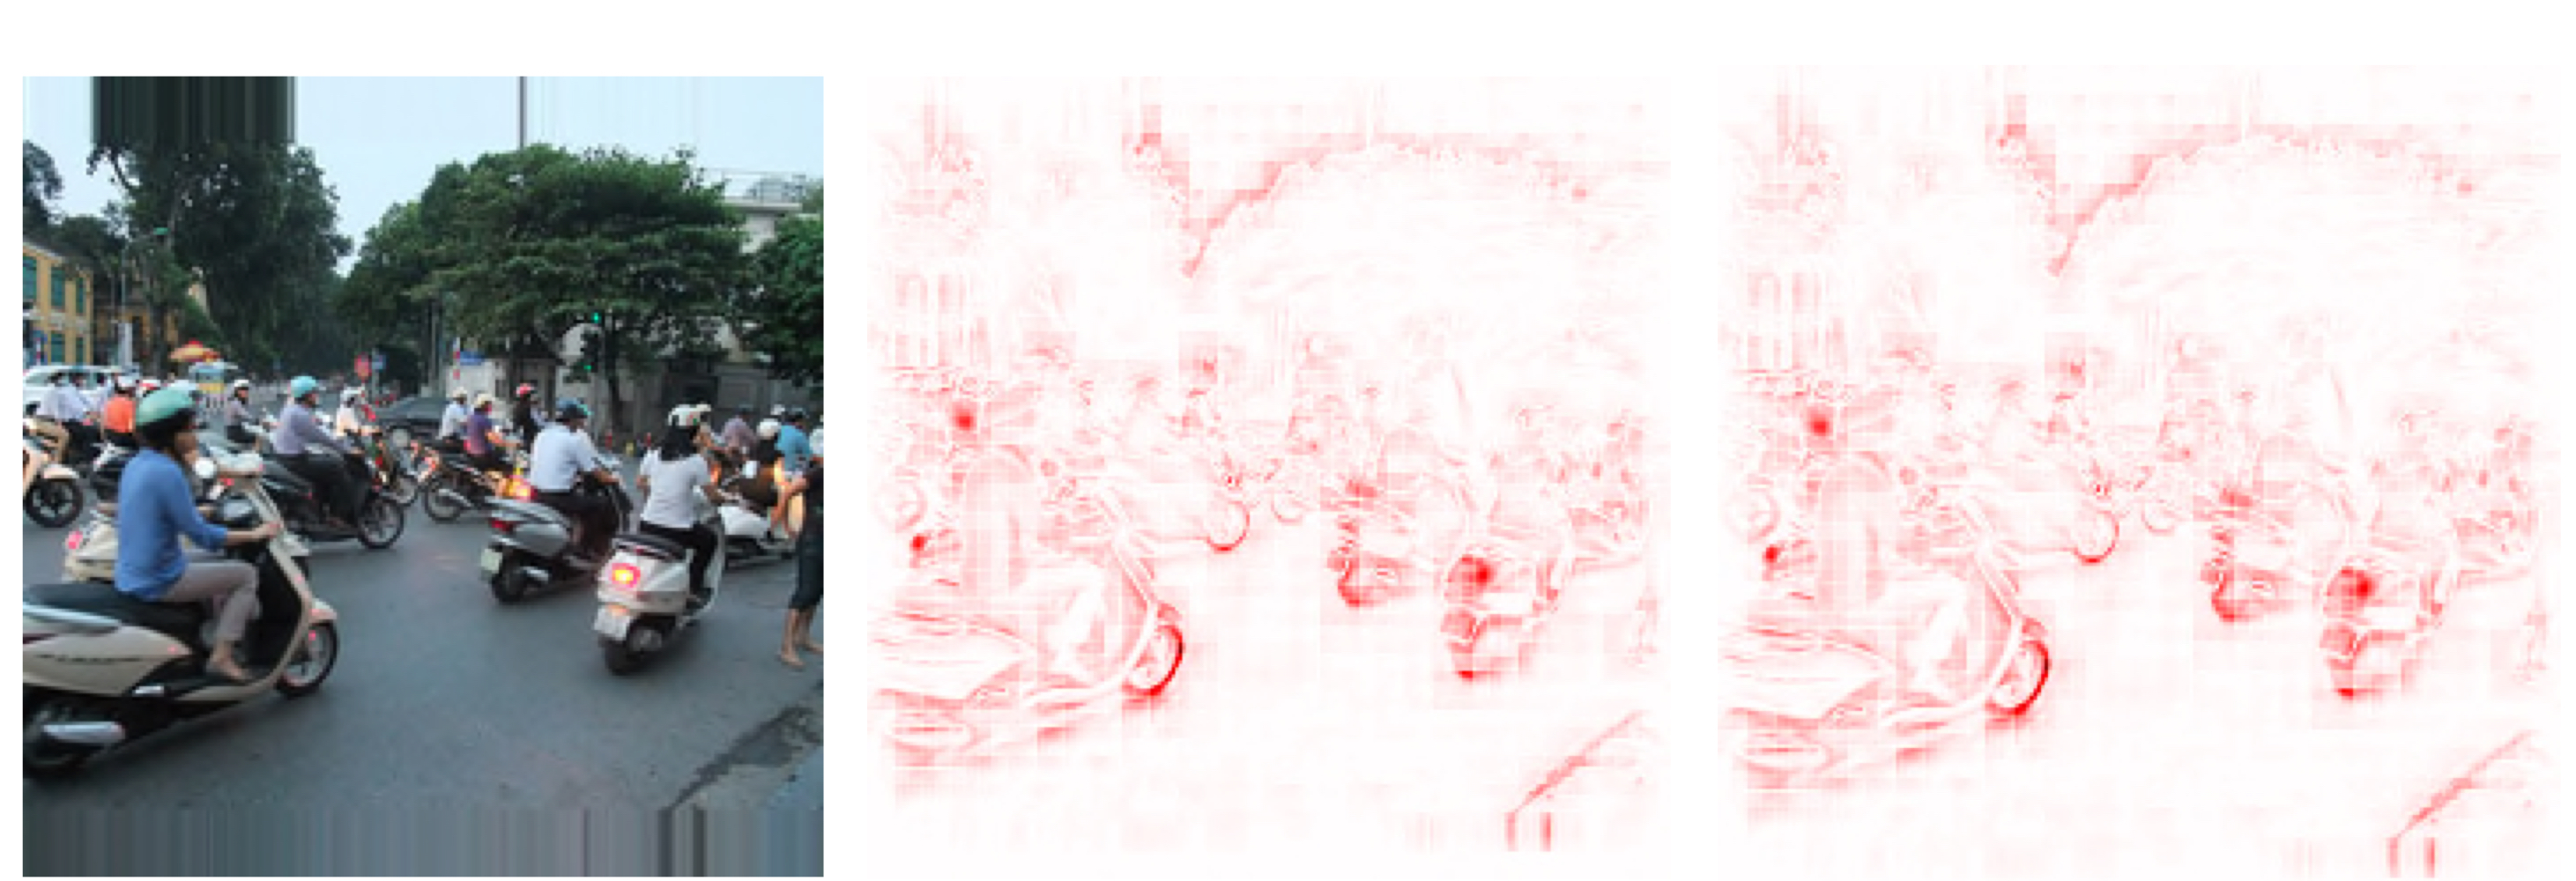
\includegraphics[width=0.65\textwidth]{grafiken_theo/expl_ai_z+.jpeg}
\caption{Implementierung der $z^+$-Regel durch Tool des Fraunhofer Instituts, angewendet auf Klassifizierung als \textit{Motorroller} und 
\textit{Motorradhelm}\footnote{https://lrpserver.hhi.fraunhofer.de/image-classification}.}
\end{figure}
\end{frame}


\section{Literatur}
\begin{frame}{Quellen}
\begin{itemize}
\item Quellen für Bilder, Implementierungshinweise:
\item Montavon, Binder, Lapuschkin, Samek, Müller :  \\
"{}Layer-Wise Relevance Propagation: An Overview"{}\\
Gefunden auf: \\
$\rightarrow$ \url{http://iphome.hhi.de/samek/pdf/MonXAI19.pdf}
\label{itm:LRPOv}
\end{itemize}
\end{frame}

\begin{frame}{Quellen}
\begin{itemize}
\item Quellen für Bilder, Implementierungshinweise:
\item Montavon et al. : \\
"{}Explaining nonlinear classification decisions with deep Taylor decomposition"{}\\
Version mit Appendix, gefunden unter:\\
$\rightarrow$ \url{https://arxiv.org/pdf/1512.02479v1.pdf}
\label{itm:Mont17}
\end{itemize}
\end{frame}

\begin{frame}{Quellen}
\begin{itemize}
\item Quellen zum weiteren Verständnis:
\item Montavon: \\
"{}Deep Taylor Decomposition, Conference Talk"{}\\
Gefunden auf: \\
$\rightarrow$ \url{https://www.youtube.com/watch?v=gy_Cb4Do_YE&t=939s}
\label{itm:MontTalk}
\item Montavon, Samek, Müller:  \\
"{}Methods for interpreting and understanding deep neural networks"{}\\
Gefunden auf: \\
$\rightarrow$ \url{https://doi.org/10.1016/j.dsp.2017.10.011}
\label{itm:MethodsPaper}
\end{itemize}

\end{frame}


%\include{content_bonus}

\end{document}